\section{Supplementary Studies}\label{sec:supplementary_studies}

In this section, we bring the following supplementary preliminary evaluations
and open topics concerning the \rnn{}: the development of \rnn{} for the
selection of electrons with $\et<\SI{15}{\GeV}$ (Section~\ref{ssec:low_et}), the
selector efficiency when only \ecal{} information is employed
(Section~\ref{ssec:ecal_rnn}), some lumiblocks with possible inconsistent
trigger efficiencies (Section~\ref{ssec:lbs_lower_eff}) and additional
evaluations concerning the agreement analysis
(Section~\ref{ssec:supplementary_agreement}).

\subsection{\rnn{} for Triggering on Electrons Below \SI{15}{\GeV}}%
\label{ssec:low_et}

We employed the 2018 tuning strategy (Section~\ref{ssec:2018}) to derive
expert MLPs for the lower kinematic region, but with some
adaptations. First, the signal event selection employs the \Jee{} \tnp{}
method~\cite{PERF-2016-01}.  Likewise, we employ full\footnote{Requiring events
within the latest GRLs available in the start of 2019.} 2017 and 2018 data to
derive the tunes. The \abseta{} bins are the same as in the \Zee{} \tnp{} tunes,
but the \et{}~$[\GeV]$ bins are delimited by $\{3,7,10,15\}$. The 15 expert MLPs (3 in
\et{} $\times$ 5 in \eta{}) derived with \Jee{} \tnp{} data are joined to those
derived with \Zee{} \tnp{} to build a single ensemble comprising the full
kinematic range employed for trigger selection. The selection of the expert MLP
to operate does not account for the trigger energy-threshold, therefore a
\SI{5}{\GeV} threshold trigger selects a MLP trained with \Zee{} data if the
electron candidate has $\et{} > \SI{15}{\GeV}$ when reconstructed by the
\fastcalo{}.

% Tuning strategy
The Figures~\ref{fig:lowet_e5_lhloose_bkg} and~\ref{fig:lowet_e5_lhloose} show
the \rnn{} trigger operating with same signal efficiency for the \loose{}
working point. It results in a considerable reduction in the \fastcalo{}
fake rate ($4.2\;\times$: \SI{34.71}{\%}$\rightarrow$\SI{5.64}{\%}), depicted as a function of
\eta{} in Figure~\ref{fig:lowet_e5_lhloose_bkg}. This reduction in the fake rate
is of $1.3\;\times$ (\SI{0.25}{\%}$\rightarrow$\SI{0.19}{\%}) in the \hlt{}. In
case it directly impacts the trigger output rates\footnote{Recall that the
impact in the fake rate when measured with respect to the offline did
not reflect in output rate improvements for the lowest-threshold unprescaled
single electron trigger (see Section~\ref{ssec:2017}).}, it might allow to
reduce triggers applying HLT prescale factor to, in the optimistic scenario,
$\SI{75}{\%}$ of its original value and result in more interesting data volume
collected. However, most interesting triggers with electron legs below
\SI{15}{\GeV} are prescale factors applied only in L1.

\begin{figure}[b]
  \centering
  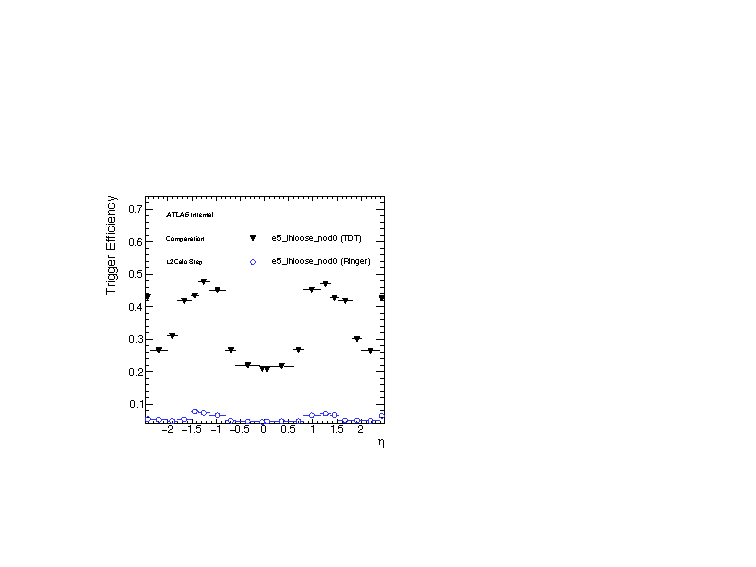
\includegraphics[width=.5\textwidth]{appendices/figures/low_et/e5_lhloose_eta_bkg}
  \caption{\label{fig:lowet_e5_lhloose_bkg}
\fastcalo{} background efficiency as a function of \eta{} for an electron
trigger requiring $\et > \SI{5}{\GeV}$ and \loose selection with (blue) and
without (black) the \rnn algorithm. Samples are selected with \Jee{} \tnp{} and
efficiencies are measured with full 2017 data employing the TriggerDecisionTool
(TDT) framework for the trigger without \rnn{}. The full trigger selection is
emulated on the same samples with the TriggerEmulationTool framework to allow
estimating the efficiency of the trigger with \rnn{}.
}
\end{figure}

\begin{figure}[htb]
\begin{center}
\begin{subfigure}[c]{.48\textwidth}
\centering
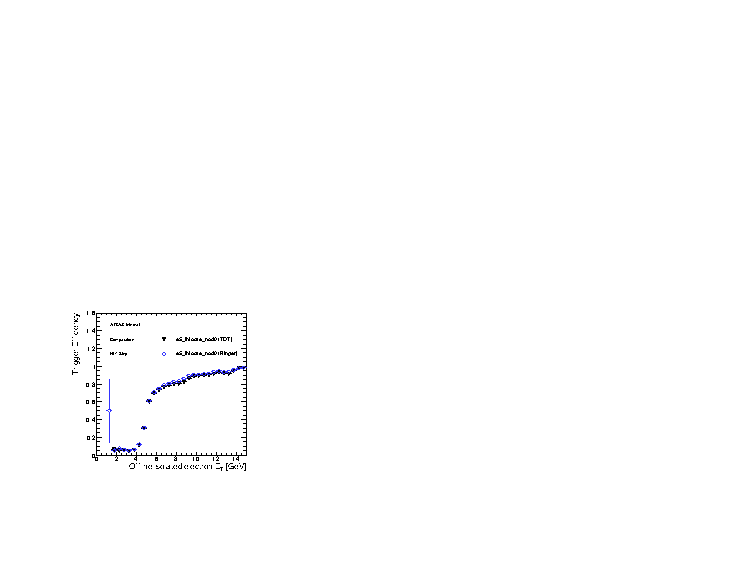
\includegraphics[width=\textwidth]{appendices/figures/low_et/e5_lhloose_et}
\caption{}
\label{fig:lowet_comp_et}
\end{subfigure}
\hfill
\begin{subfigure}[c]{.48\textwidth}
\centering
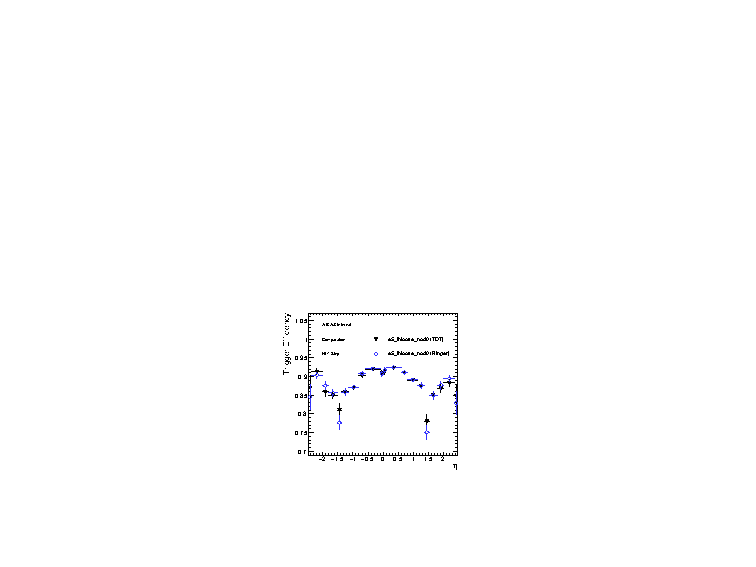
\includegraphics[width=\textwidth]{appendices/figures/low_et/e5_lhloose_eta}
\caption{}
\label{fig:lowet_comp_eta}
\end{subfigure} \\
\begin{subfigure}[c]{.48\textwidth}
\centering
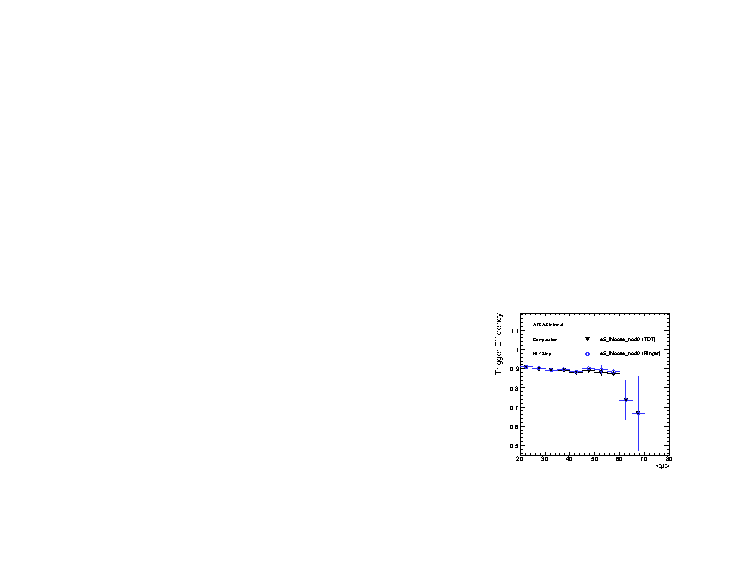
\includegraphics[width=\textwidth]{appendices/figures/low_et/e5_lhloose_mu}
\caption{}
\label{fig:lowet_comp_mu}
\end{subfigure}
%\hfill
\caption{HLT electron efficiency as a function of \et{} (a), \eta{} (b) and \avgmu{}
(c) for an electron trigger requiring $\et > \SI{5}{\GeV}$
and \loose selection with (blue) and without (black) the \rnn algorithm. Details
on the efficiency measurement are described in
Figure~\ref{fig:lowet_e5_lhloose_bkg}.
}%
\label{fig:lowet_e5_lhloose}
\end{center}
\end{figure}

\FloatBarrier
\subsection{\rnn{} based only on ECAL Information}%
\label{ssec:ecal_rnn}

Another limitation for online operation is the trigger system readout
capability. Particularly, the readout rate of the \hcal{} cells is more likely
to reach its limitations given the hadronic pile-up nature and the their coarser
granularity. Some electron triggers, as those dedicated to cover
\BeeK{} decays, may be executed on top of the full \licalo{}
rate. A main challenge for these triggers during Run~2 was the \hcal{} readout
rate, which triggered the interest of developing an electron selection based only
in the \ecal{} information~\cite{ATR-18724}. It may be noticed that for low
kinematic operation (i.e. $\et<\SI{15}{\GeV}$) the signal-to-noise ratio in the
\hcal{} is lower due to pile-up contamination and, thus, may not be as useful as
for the selection of higher \et{} physics objects.

When investigating how much the hadronic information was beneficial to the
selector at the low kinematic region (Table~\ref{tab:comp_ecal_rnn}), we
observed that the \rnn{} operating with only \ecal{} information can bring
similar improvements with respect to the cut-based strategy. Depending on the
working point, a reduction of 25--50$\;$\% with respect to triggering without
\rnn{} can be obtained in the \fastcalo{} fake rate, while keeping the same
signal efficiency. If needed to keep the full \rnn{} efficiency, a possible
strategy could be to apply a two step \fastcalo selection, starting with the
\ecal{} and then applying the full \rnn{} decision. Finally, the \BeeK{} trigger
requires \rnn{} to handle boosted physics structure, which is part of the open
topics (Section~\ref{ssec:boosted_topology}).

\begin{table}[htb]
  \centering
  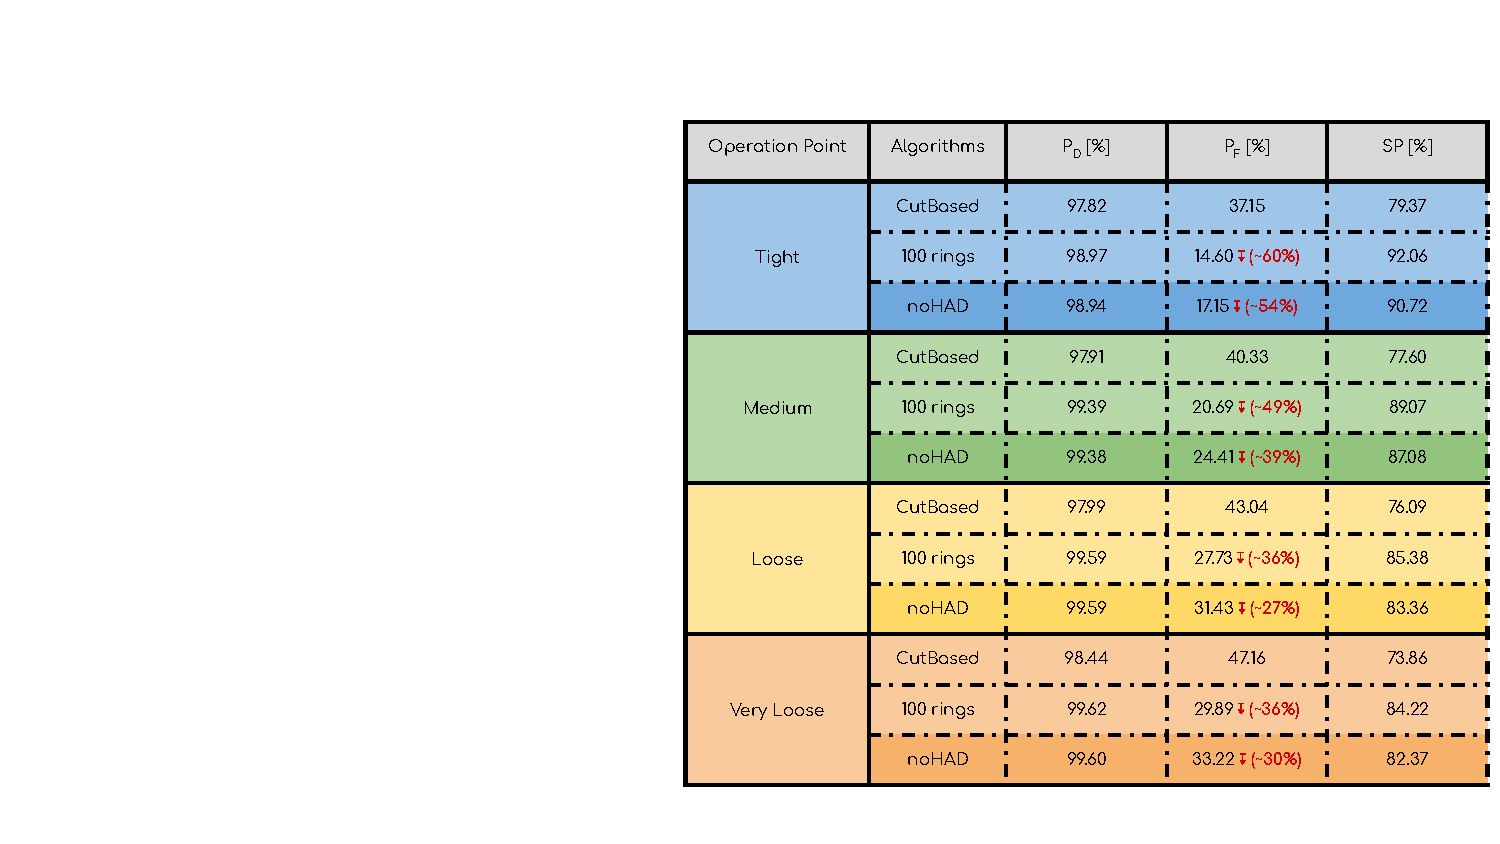
\includegraphics[width=.65\textwidth]{appendices/figures/low_et/nodhad_comparison_with_cutbased}
  \caption{Algorithm efficiencies for each working point using joint 2017 and
    2018 data as described in Section~\ref{ssec:low_et}. The fraction of fake
    rate reduction with respect to the cut-based algorithm is shown in red.
    `noHAD' is used to flag the \rnn{} algorithm accessing only \ecal{}
    information, whereas `100 rings' is the standard version of the \rnn{}.
  \label{tab:comp_ecal_rnn}}
\end{table}

%\subsection{Fudge Factors}%
%\label{ssec:fudge_factors}
% TriggerEgammaMeeting_20180213

\subsection{Lumiblocks with Inconsistent Trigger Efficiency}\label{ssec:lbs_lower_eff}
%/Users/wsfreund/Documents/Pesquisa/HEP/CERN/ID/Online/impact_on_lhpdfs/2017data/e28/runsSummaryLB_e28.pdf

By evaluating the number of \Zee{} \tnp{} pairs as in
Figure~\ref{fig:tap_pairs_count}, it is possible to observe some luminosity
blocks (LBs) where the trigger collect potentially less pairs than what was 
expected\footnote{The particular plot may be interesting to be implemented for
online and data quality monitoring. For instance, Figure~\ref{fig:run335282}
shows some LBs within the GRL where the \Zee{} \tnp{} electron trigger
efficiency was very low and may be worth the investigation for data quality
purposes.}.  Particularly, the LBs 113--136 in run 327636
(Figure~\ref{fig:run327636}), the range near 100--180 in run 328636
(Figure~\ref{fig:run328636}) and near 120--160 in run 331975
(Figure~\ref{fig:run331975}) show lower number of pairs with respect to the
other LBs for both duplicated triggers. For the particular regions, the trigger
with \rnn{} has a slightly lower number of pairs with respect to the its
cut-based counterpart. Investigating these data might improve the detection of
possible detector anomalies, but also it brings insights of the particularities
between the algorithms. Likewise, LBs 501, 751 and 790 in run 334779
(Figure~\ref{fig:run334779}) might be showing a systematic behavior where the
trigger with \rnn{} has higher efficiency than its counterpart.


\begin{figure}[b]
  \centering
\begin{subfigure}[c]{.49\textwidth}
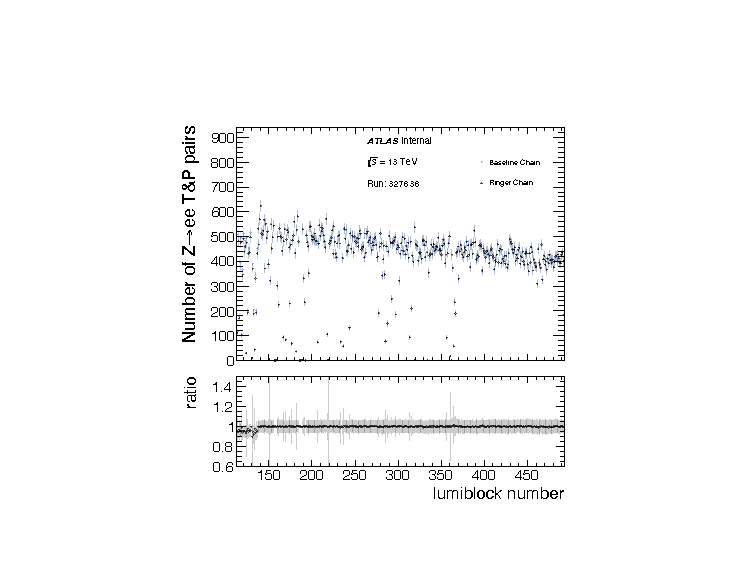
\includegraphics[width=\textwidth]{appendices/figures/pairs_wrt_lb/run327636}%
\caption{\label{fig:run327636}}
\end{subfigure}
\hfill
\begin{subfigure}[c]{.49\textwidth}
\centering
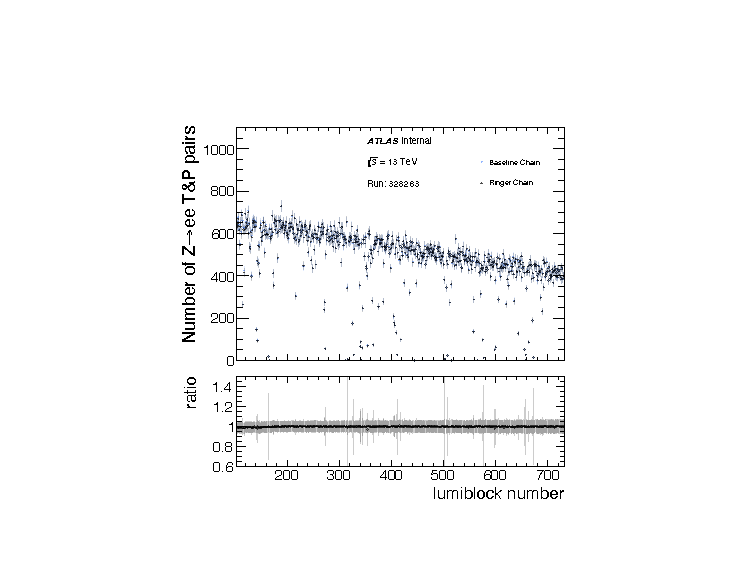
\includegraphics[width=\textwidth]{appendices/figures/pairs_wrt_lb/run328263}%
\caption{\label{fig:run328636}}
\end{subfigure} \\
%\end{figure}
%\begin{figure}[t]\ContinuedFloat
\centering
\begin{subfigure}[c]{.49\textwidth}
\centering
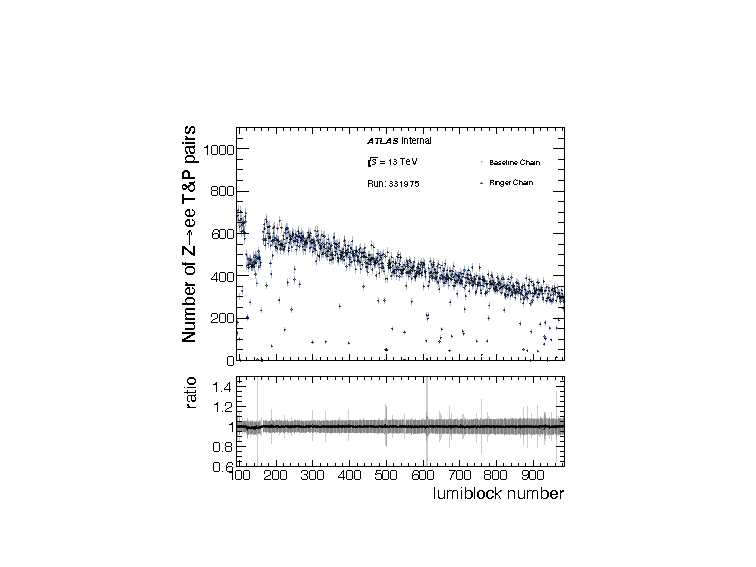
\includegraphics[width=\textwidth]{appendices/figures/pairs_wrt_lb/run331975}%
\caption{\label{fig:run331975}}
\end{subfigure}
\hfill
\begin{subfigure}[c]{.49\textwidth}
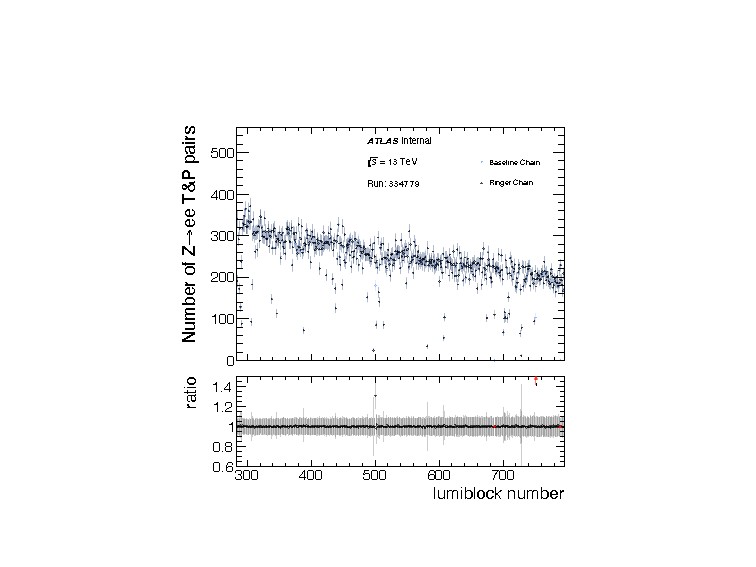
\includegraphics[width=\textwidth]{appendices/figures/pairs_wrt_lb/run334779}%
\caption{\label{fig:run334779}}
\end{subfigure} \\
\begin{subfigure}[c]{.30\textwidth}
\centering
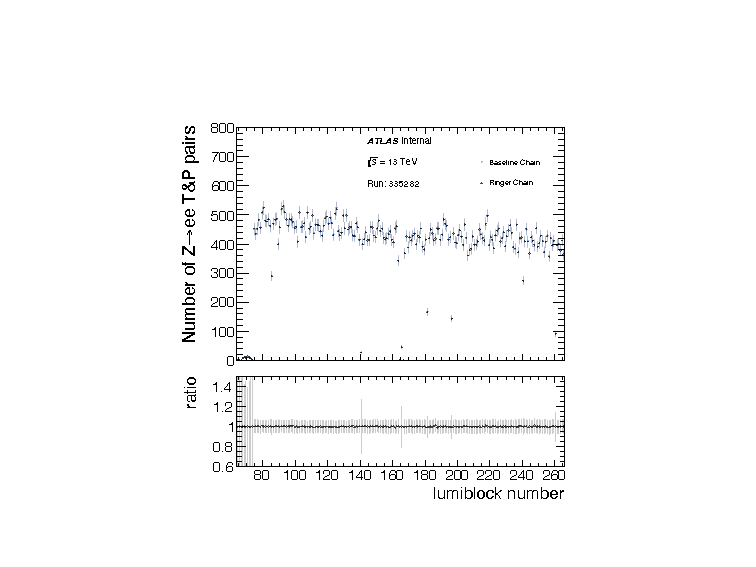
\includegraphics[width=\textwidth]{appendices/figures/pairs_wrt_lb/run335282}%
\caption{\label{fig:run335282}}
\end{subfigure}
\caption{\label{fig:tap_pairs_count}
Number of \Zee{} \tnp{} pairs collected by the duplicated trigger with (blue)
and without (black) \rnn{} per luminosity block in the good run list (GRL)
for five runs (from (a) to (e)) along 2017 data-taking.
}
\end{figure}

%\FloatBarrier{}
%\subsection{On-going Evaluations on the Quadrant Analysis}\label{ssec:quadrant_combined}
%
%An asymmetry can be observed in \deltaeta{} when we consider the
%disagreement profiles (Figure~\ref{fig:trigger_quadrant_deltaEta}), where the
%trigger with (without) \rnn{} is biased towards collecting more samples with
%negative (positive) value. This behavior only happens for the
%$0.6<\abseta{}<0.8$ region.
%
%\rnn{} trigger also displays a slightly less pronounced tail in \deltaphi{}
%(Figure~\ref{fig:trigger_quadrant_deltaPhi}).  Hence, there is some correlation
%level between this variable and the shower development information being
%explored by the \rnn{} algorithm.
%
%\begin{figure}[h!tb]
%\begin{subfigure}[c]{.49\textwidth}
%\includegraphics[width=\textwidth]{quadrant_plots/HLT_e28_lhtight_nod0_noringer_ivarloose_HLT_e28_lhtight_nod0_ivarloose_deltaEta1_et4_eta1.pdf}%
%\caption{\label{fig:trigger_quadrant_deltaEta}}
%\end{subfigure}
%\hfill
%\begin{subfigure}[c]{.49\textwidth}
%\centering
%\includegraphics[width=\textwidth]{quadrant_plots/HLT_e28_lhtight_nod0_noringer_ivarloose_HLT_e28_lhtight_nod0_ivarloose_deltaPhiRescaled2_et4_eta1.pdf}%
%\caption{\label{fig:trigger_quadrant_deltaPhi}}
%\end{subfigure} \\
%\caption{\label{fig:quadrant_combined_variables_30GeV}
%Quadrant analysis plots for the offline-reconstructed ID-calorimeter combined
%variables employed in the likelihood for the $0.6<\abseta{}<0.8$ and
%$30<\et{}~[\text{GeV}]<35$ slice.
%}
%\end{figure}
%
\FloatBarrier
\subsection[Supplementary Agreement Analysis]{Supplementary Agreement
Analysis\footnote{Figures shown in this section may not contain the
`\textbf{ATLAS} \emph{Internal}' label as the only version available was
created to be part of a PhD thesis but we emphasize that these figures have
not been approved as ATLAS public plots. Their regeneration to include the
internal flag is not straightforward.}}\label{ssec:supplementary_agreement}


Current tools available in physics data analysis frameworks provide statistical
tests that, although they have not been designed to the conditions of the
agreement analysis, can provide some useful insights. We take advantage of these
tests in one approach complementary to the homogeneity test presented in
Section~\ref{ssec:agreement}. Additionally, we develop a simple approach based
on pseudo-experiments with ``Toy'' Monte Carlo. Such complementary studies
comply with the ATLAS statistical guideline~\cite{atlas_recommendations_stats}:

\begin{quote}
\textbf{Recommendation}: Use multiple statistical techniques. When they agree
we are in ‘asymptopia’; when they disagree we learn something.
\end{quote}

The first supplementary strategy goes in a similar direction of the baseline
evaluation (Section~\ref{top:agreement_homogeneity_results}) but, instead of
splitting data into two groups, we obtain the profiles for the two trigger
configurations for the full dataset. We approach the problem as a
goodness-of-fit problem by assuming the trigger without the \rnn{} algorithm as
a model to explain the observations obtained in the histogram built from the
trigger with the \rnn{} algorithm. For evaluating the goodness-of-fit, we employ
the Kolmogorov-Smirnov (KS)~\cite{kendalls_vol1} and
$\chi^2$~\cite{guide_to_chisquared} tests.

The small differences in efficiency between the triggers result in fluctuations
in the number of probes in the histograms (see
Appendixes~\ref{top:homogeneity_extra} and~\ref{top:gof_extra}). Instead
reweighing the histograms to have the same mass, we preferred to keep the
original histograms and compute the expected $\chi_{i,j}^{s}$ residuals by

\begin{equation}
  \frac{\mu_{i,j}}{\sigma_{ref}} = \frac{\left(r_j - b_j\right) \times
  \frac{b_{i,j}}{b_i}}{\sigma_{b_{i,j}}},
  \label{eq:expected_residual}
\end{equation}

\noindent where $r_j$ and $b_j$ are the total number of observations in the
$j$th histograms obtained with and without ringer. $\sigma_{b_{i,j}}$ will be
employed as a unit for measuring the residuals. In order to benefit from
Gaussian error approximation ($\sigma_{b_{i,j}}\approx\sqrt{b_{i,j}}$), we
employed the conservative recommendations in~\cite{knoll} by grouping the
histogram bins to have a minimum count of 30 units. Results are available in
Section~\ref{top:agreement_gof_results}.

Finally, we dedicate to the direct evaluation of possible distortions in the
profiles by considering only the disjoint cases where the triggers with and
without \rnn{} disagree. To consider the dependency of the duplicated
trigger pair, we adopted a pseudo-experiment strategy using simulation.
Considering that both disjoint histograms come from the same population, we can
estimate the original profile based on maximum
likelihood as~\cite{chi_squared_comparing_hists}

\begin{equation}
  \hat{p_{i,j}}=\frac{r_{i,j}+b_{i,j}}{r_i+b_i},
\end{equation}

\noindent where $r_i$ ($b_i$) represent the total observed entries of the
histogram built with data collected by the trigger with (without) \rnn{} in the
$i$th $\et{}\times\eta{}$ axis region.

% FIXME quote the number of pseudo-experiments (i.e. arXiv:1005.1891v3)

We generate $10^5$ pseudo-experiments using the estimated
probabilities and total histogram counts to compute the Kullback-Leibler
divergence (\dkl{})~\cite{2009_cichocki_nonnegative}

\begin{equation}
\dkl(p_i||q_i) = \sum\limits_{j} (p_{i,j}-q_{i,j})\ln\left(\frac{p_{i,j}}{q_{i,j}}\right),
\end{equation}

\noindent where $p$ and $q$ are distributions for each variable obtained when
employing respectively the trigger with and without the \rnn{} selection and
approximated with the empirical frequency values  The $j$th individual
contributions computed to obtain the \dkl{} are kept in order to allow
evaluation of the regions bringing larger profile distortions.  We address the
results in Section~\ref{top:agreement_pseudo_results}.

\subsubsection{Goodness-of-Fit Results}\label{top:agreement_gof_results}

Figure~\ref{fig:gof_calo} show the residuals for the goodness-of-fit approach.
When comparing it with Figure~\ref{fig:groups_homogeneity_calo},
it can be observed that the goodness-of-fit approach show much lower
residual fluctuations. Namely, for the goodness-of-fit setup, the typical
fluctuations are of $\pm$\SI{0.2}{$\sigma$} around the expected residuals due to
small alteration in the trigger efficiency for their configuration (in the
particular region, slightly lower than the trigger without \rnn{}), whereas for
the homogeneity setup residuals of up to $\pm$\SI{4}{$\sigma$} can be observed.
The smaller residuals in the goodness-of-fit are caused by the difference in the
setup employed for collecting the samples. Usually, the two profiles are
collected separately, as in the homogeneity setup, in a scenario close to
independent and identically distributed (i.i.d.) sampling. Particularly, the
fluctuations are also expected to be Gaussian in this setup. In the
goodness-of-fit approach, however, the samples come from a \emph{single}
observation group which is subject to two distinct sample damaging
processes~\cite{rao1965discrete} which represent the triggers. Unlike the
i.i.d.\@ sampling, we are subject to having the \emph{exact} same samples
composing the two profiles.

Particularly, the triggers are expected to be highly correlated, as they are
designed to perform the same task with a similar pipeline. Hence, the fraction
of exact same samples in both profiles is expected to be large and, even in the
disagreement cases, some level of statistical dependency between the algorithms
can be obtained from the variables describing the shower development.
In fact, ignoring the statistical dependency between the algorithms is to assume
that the variables will not display any systematic difference between the two
algorithms.

The statistical hypothesis assumed by the KS and $\chi^2$ tests
ignore such dependency. We obtain a p-value of 1 for both tests in all
variables and regions (Appendix~\ref{top:gof_extra}), even when not reweighing
the profiles to account for the small changes in efficiencies. In other words,
the statistical and possible systematic fluctuations are too small with respect
to the expectations under the conditions assumed by the tests. Regardless of the
flaws in the tests, it allows us to highlight that any discussion concerning the
systematic impact of the configuration is bounded to a regime lower to
the expected statistical fluctuations in goodness-of-fit tests. For these tests,
the hypothesis holding is that both profiles are statistically identical.

Interestingly enough, it is possible to get some hints of deviations in the
profile by careful examination of the residuals in Figure~\ref{fig:gof_calo}.
Particularly, the profile of the trigger with the \rnn{} shows a slight shift
towards unitary \reta{}, \rphi{} and \eratio{} (i.e.\@ residuals above the
expectations in the right tail and below in the left tail). Likewise, the
profiles might also display a shift towards null \rhad{}, but it is difficult to
get any insight for \weta{}, \fI{} and \fIII{}. In order to further investigate
these effects, we dedicated to a deeper assessment available in
Section~\ref{top:agreement_pseudo_results}.

\begin{figure}[b]
\begin{center}
\begin{subfigure}[c]{.48\textwidth}
\centering
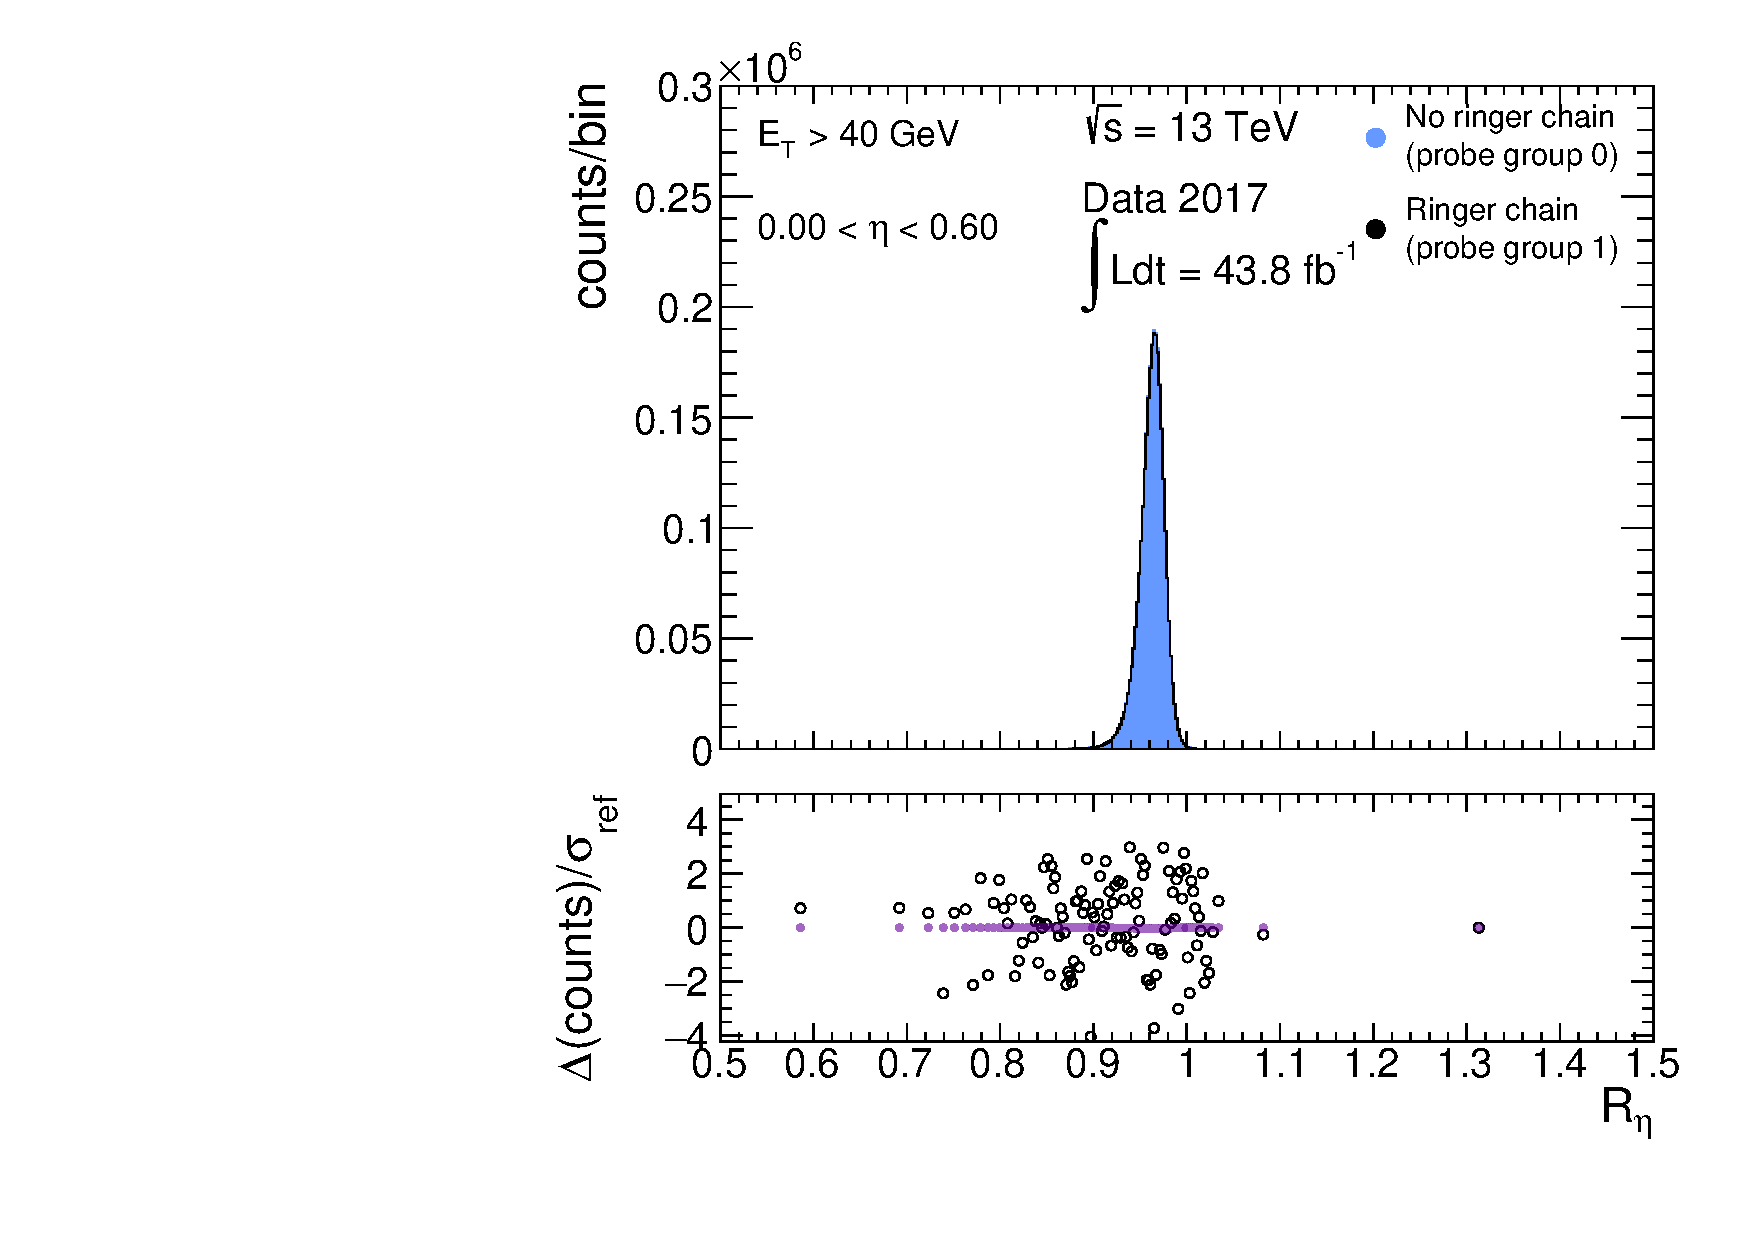
\includegraphics[width=\textwidth]{appendices/figures/noAdjustment/marginal_nosplit/e28_MergedRuns/base_new/el_reta_et40eta0_00_sigma_base_new.pdf}
\caption{}%
\label{fig:gof_reta}
\end{subfigure}
\hfill
\begin{subfigure}[c]{.48\textwidth}
\centering
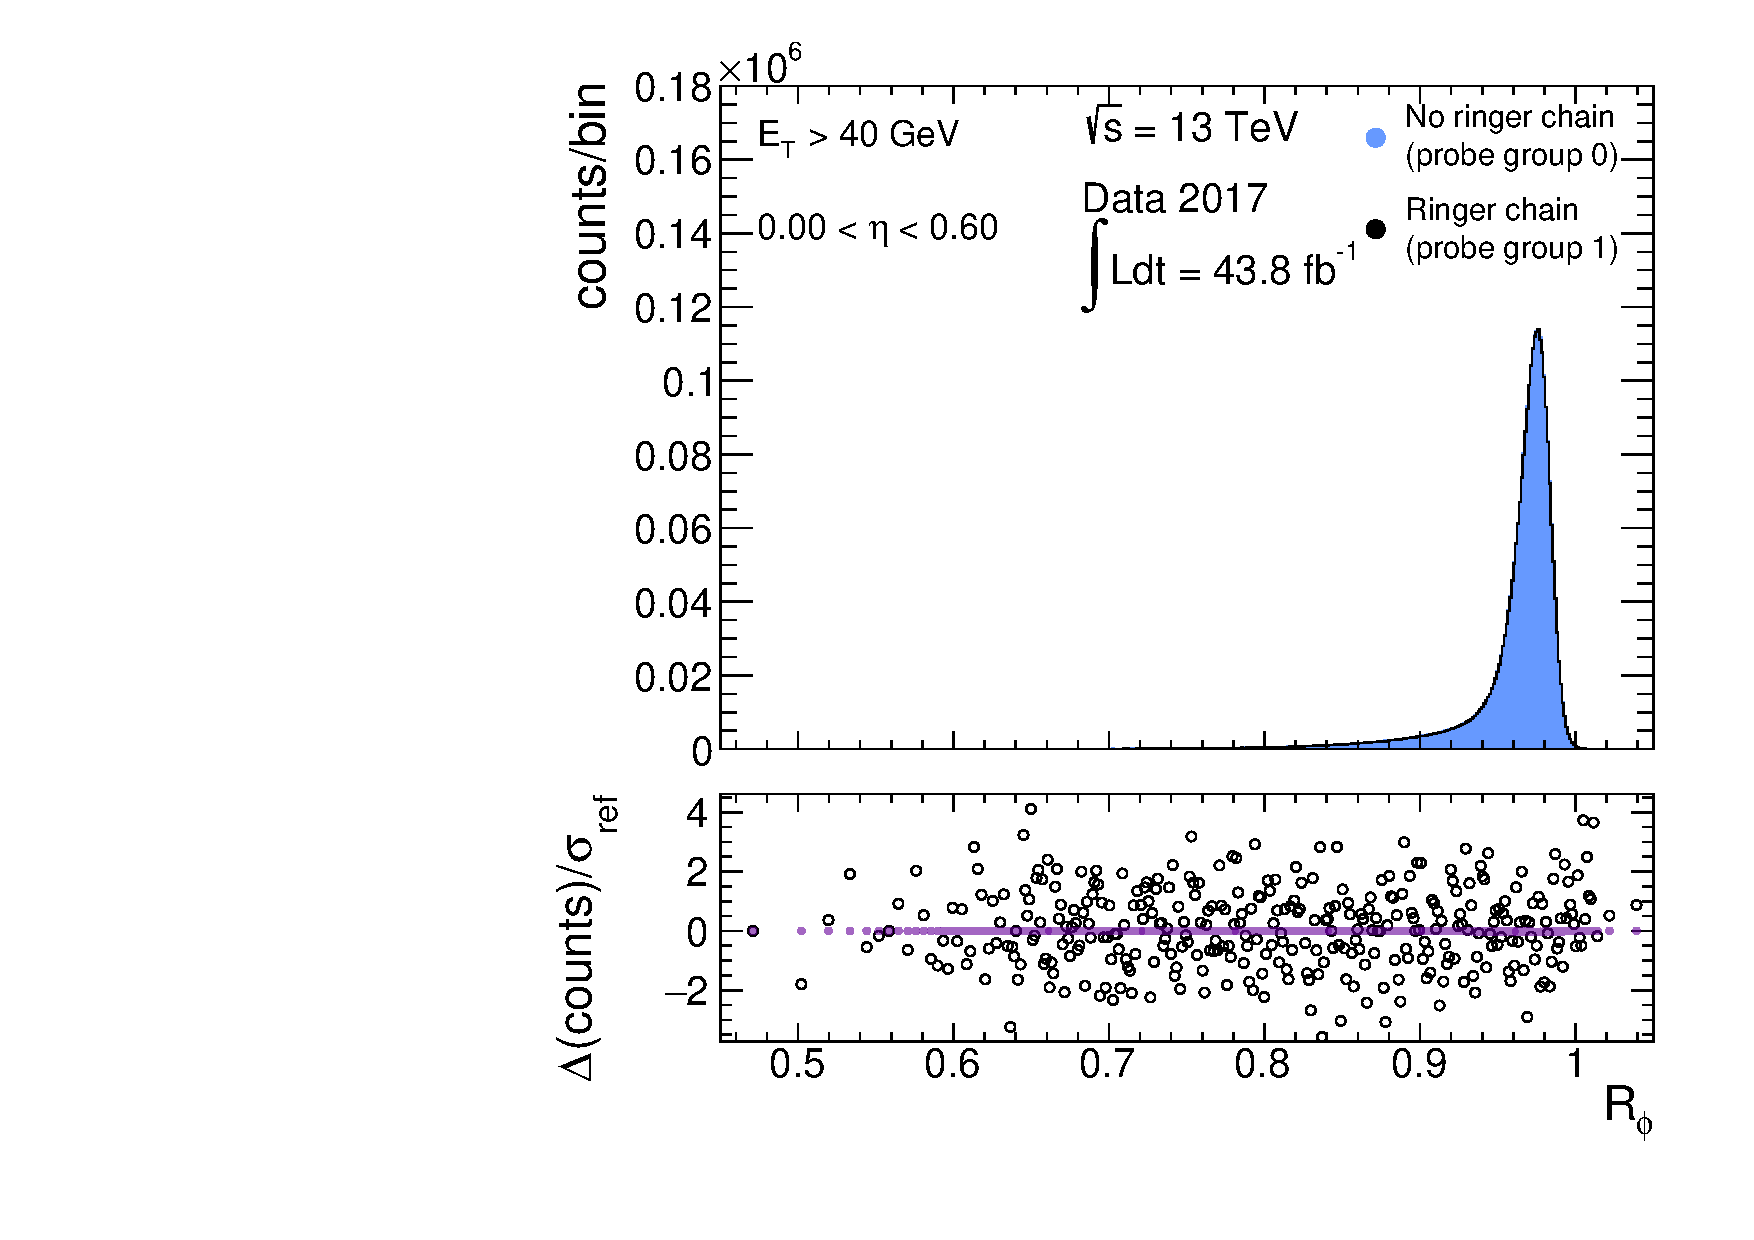
\includegraphics[width=\textwidth]{appendices/figures/noAdjustment/marginal_nosplit/e28_MergedRuns/base_new/el_rphi_et40eta0_00_sigma_base_new.pdf}
\caption{}%
\label{fig:gof_rphi}
\end{subfigure} \\
\begin{subfigure}[c]{.48\textwidth}
\centering
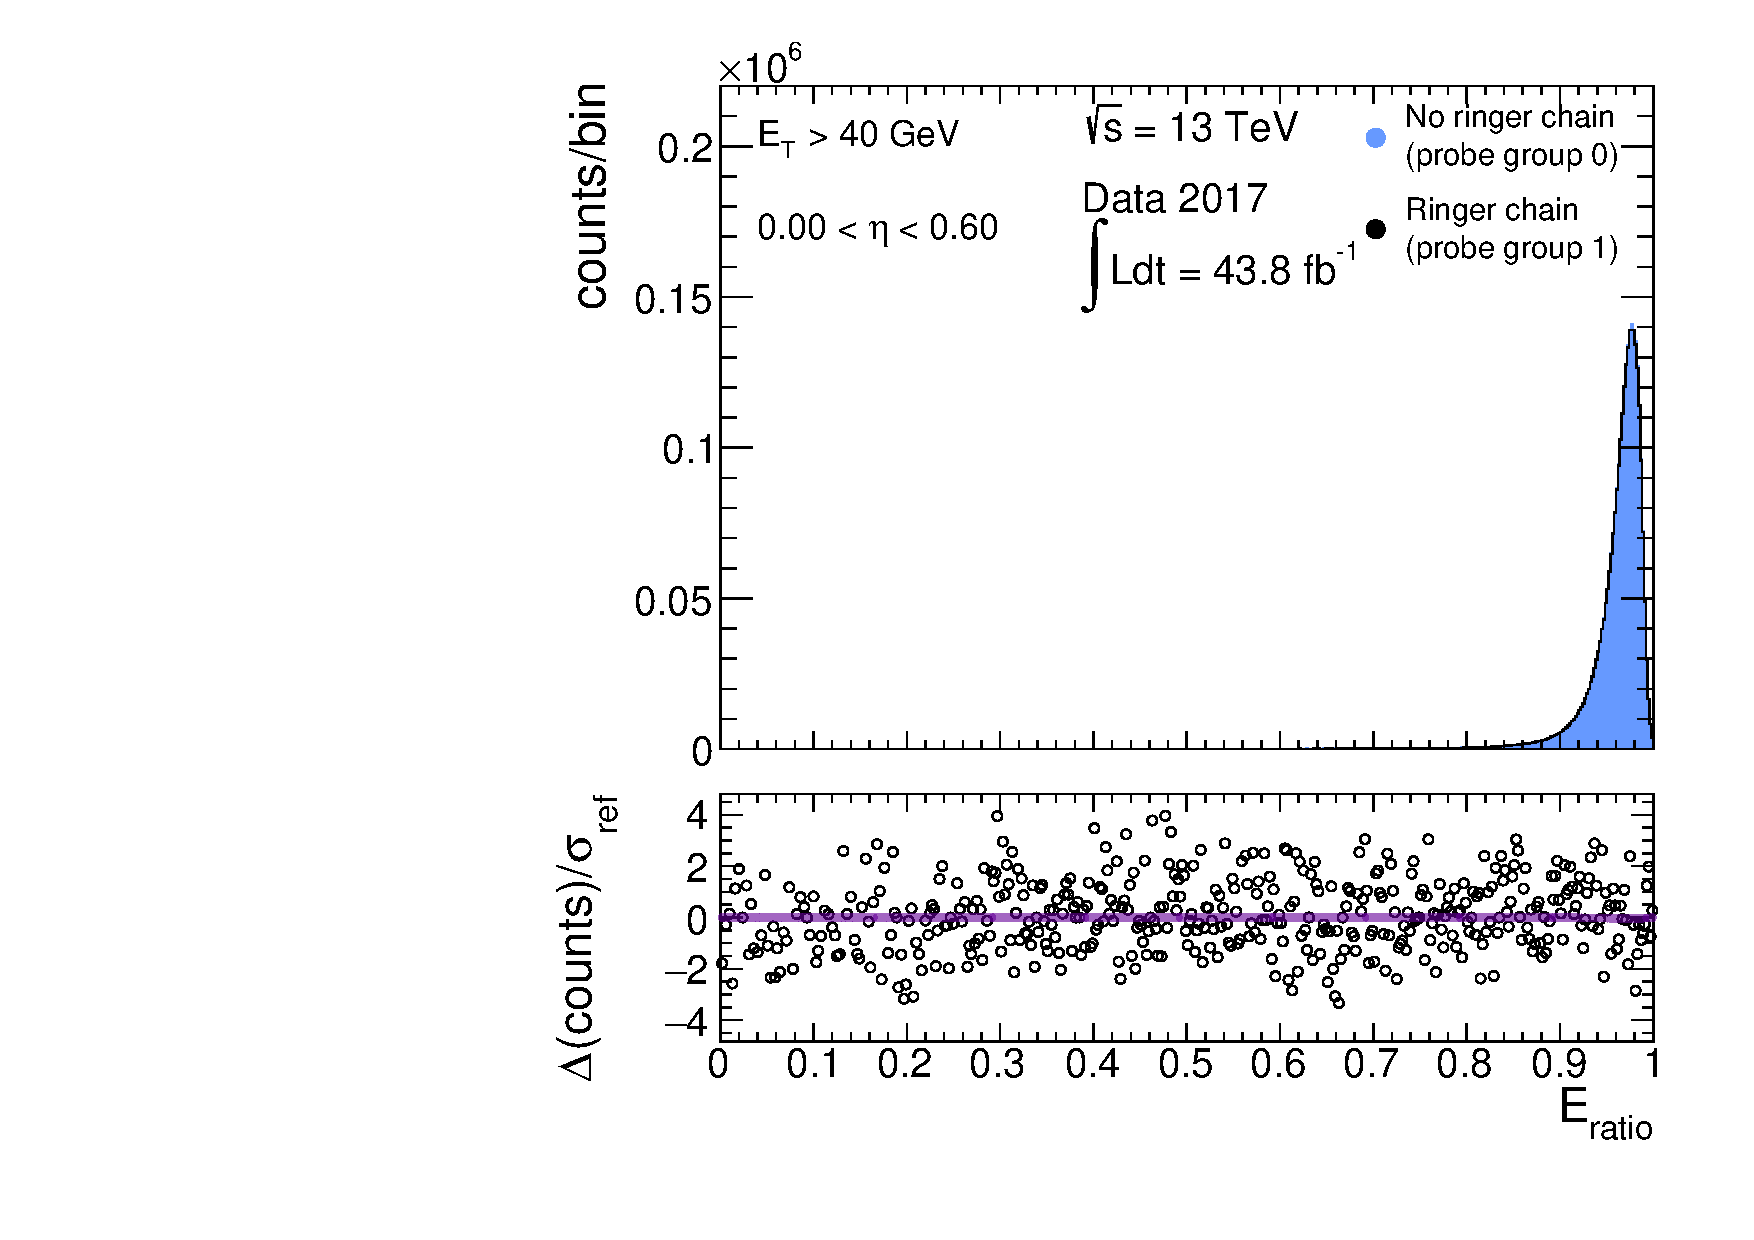
\includegraphics[width=\textwidth]{appendices/figures/noAdjustment/marginal_nosplit/e28_MergedRuns/base_new/el_eratio_et40eta0_00_sigma_base_new.pdf}
\caption{}%
\label{fig:gof_eratio}
\end{subfigure}
\hfill
\begin{subfigure}[c]{.48\textwidth}
\centering
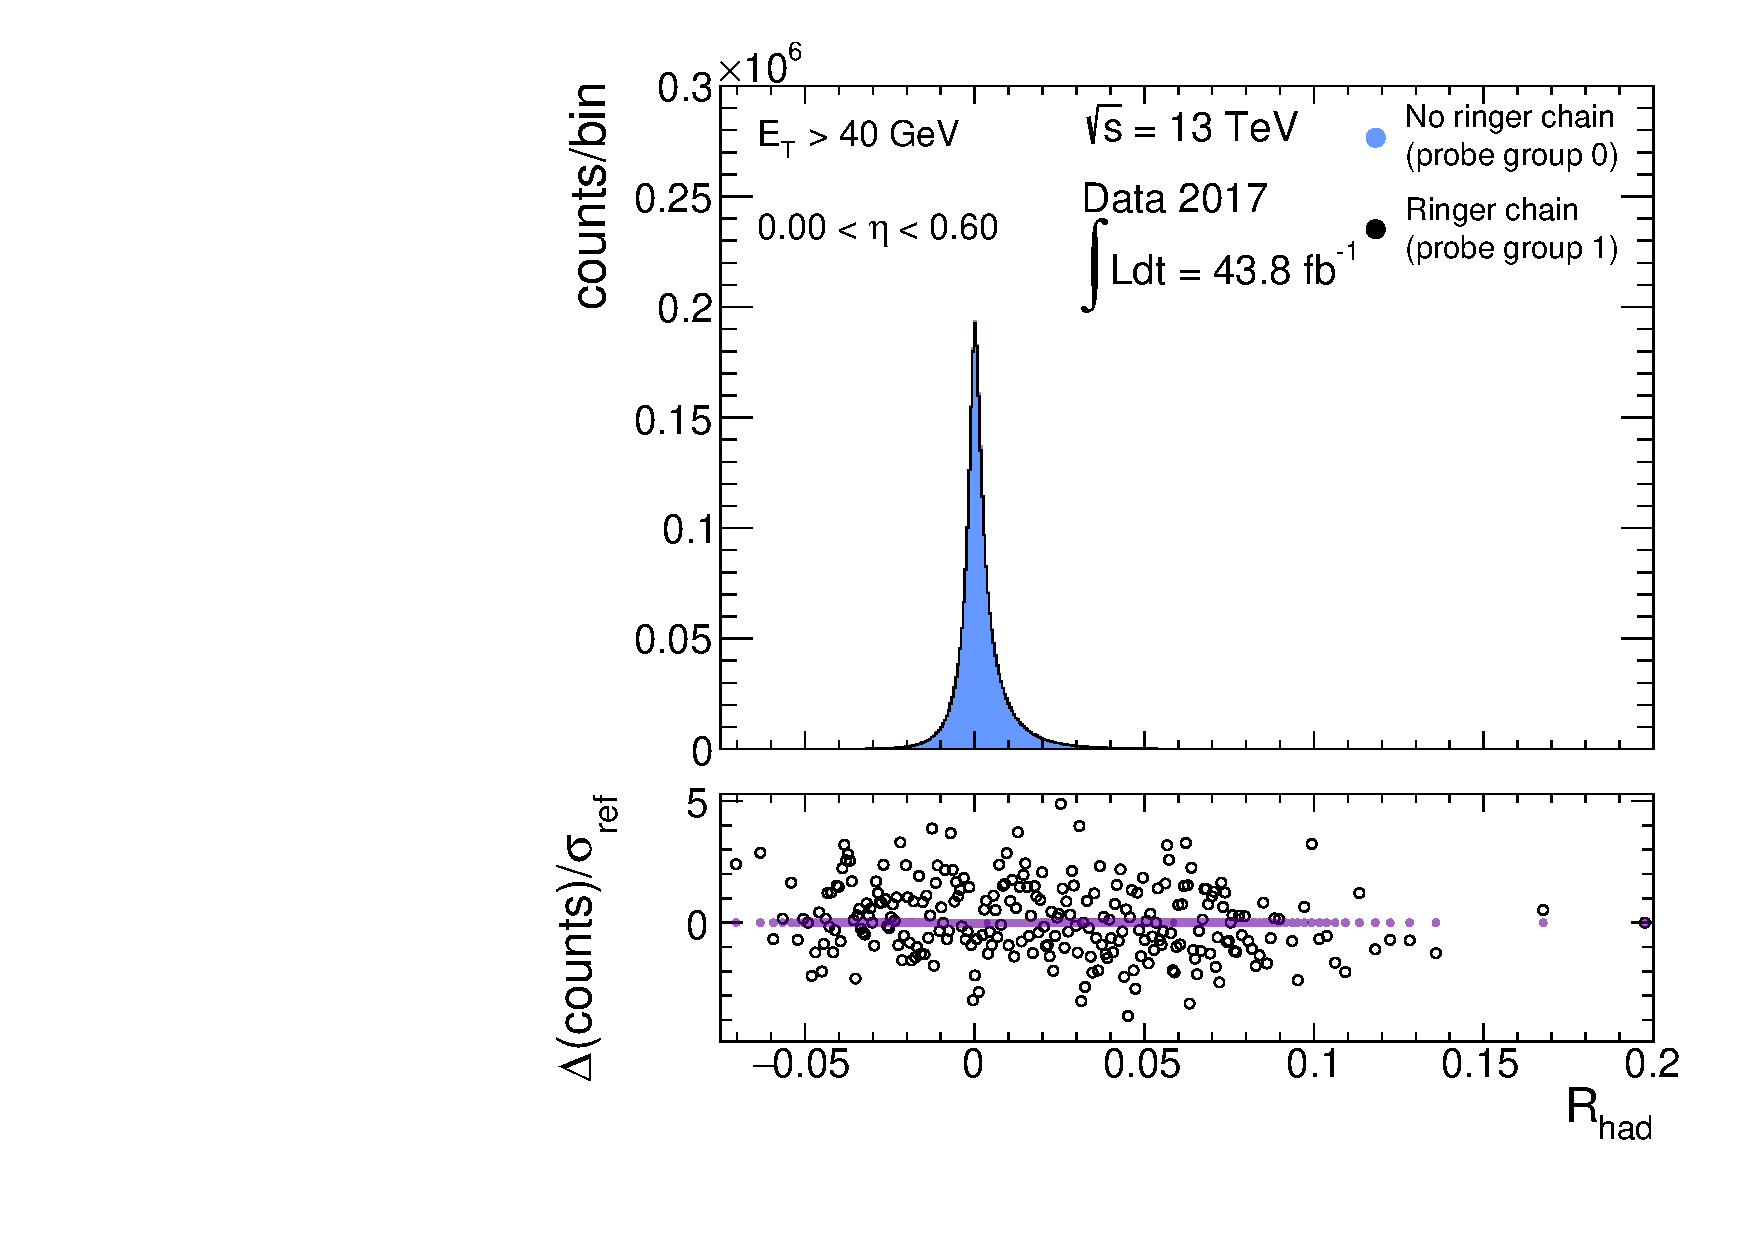
\includegraphics[width=\textwidth]{appendices/figures/noAdjustment/marginal_nosplit/e28_MergedRuns/base_new/el_rhad_et40eta0_00_sigma_base_new.pdf}
\caption{}%
\label{fig:gof_rhad}
\end{subfigure} \\
\end{center}
\end{figure}%
\begin{figure}[t]\ContinuedFloat
\begin{center}
\hspace*{\fill}
\begin{subfigure}[c]{.48\textwidth}
\centering
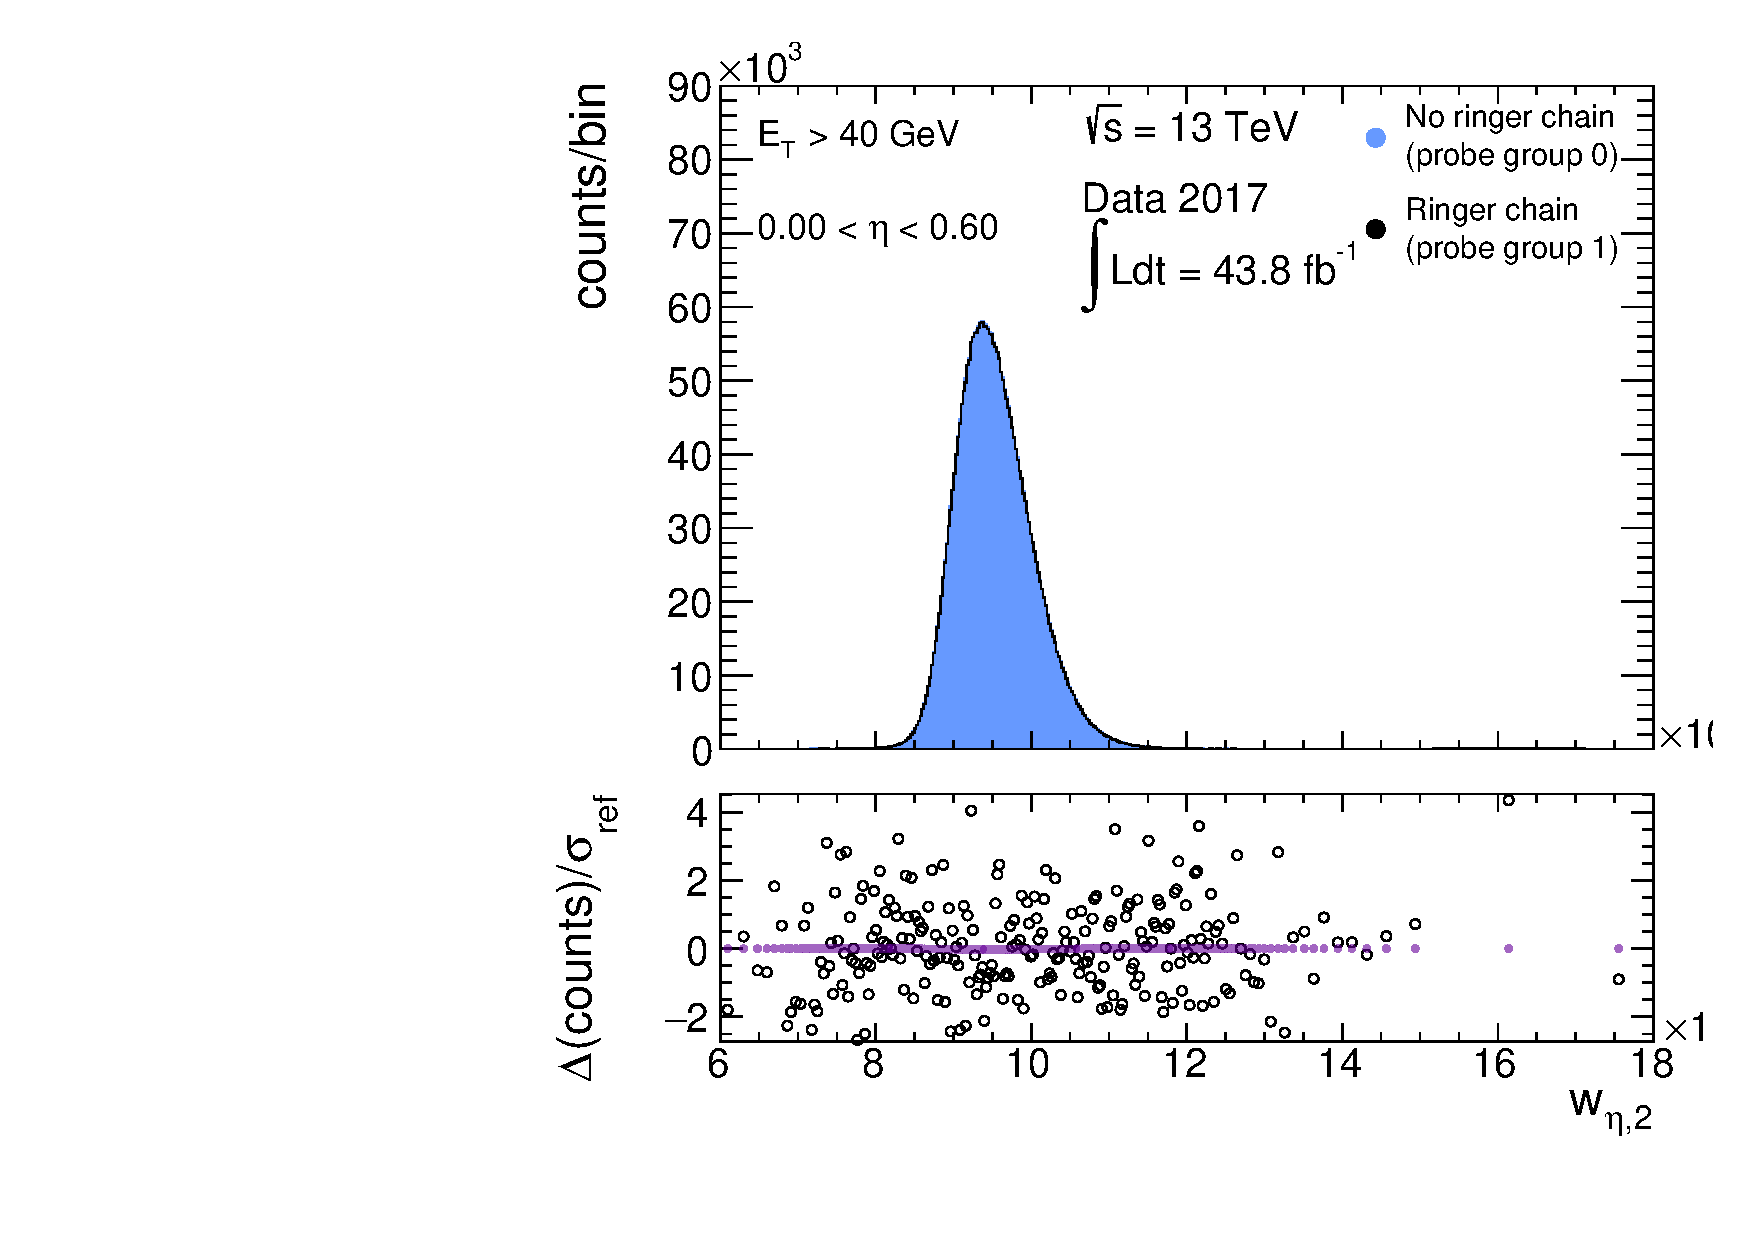
\includegraphics[width=\textwidth]{appendices/figures/noAdjustment/marginal_nosplit/e28_MergedRuns/base_new/el_weta2_et40eta0_00_sigma_base_new.pdf}
\caption{}%
\label{fig:gof_weta}
\end{subfigure}
\hspace*{\fill} \\
\begin{subfigure}[c]{.48\textwidth}
\centering
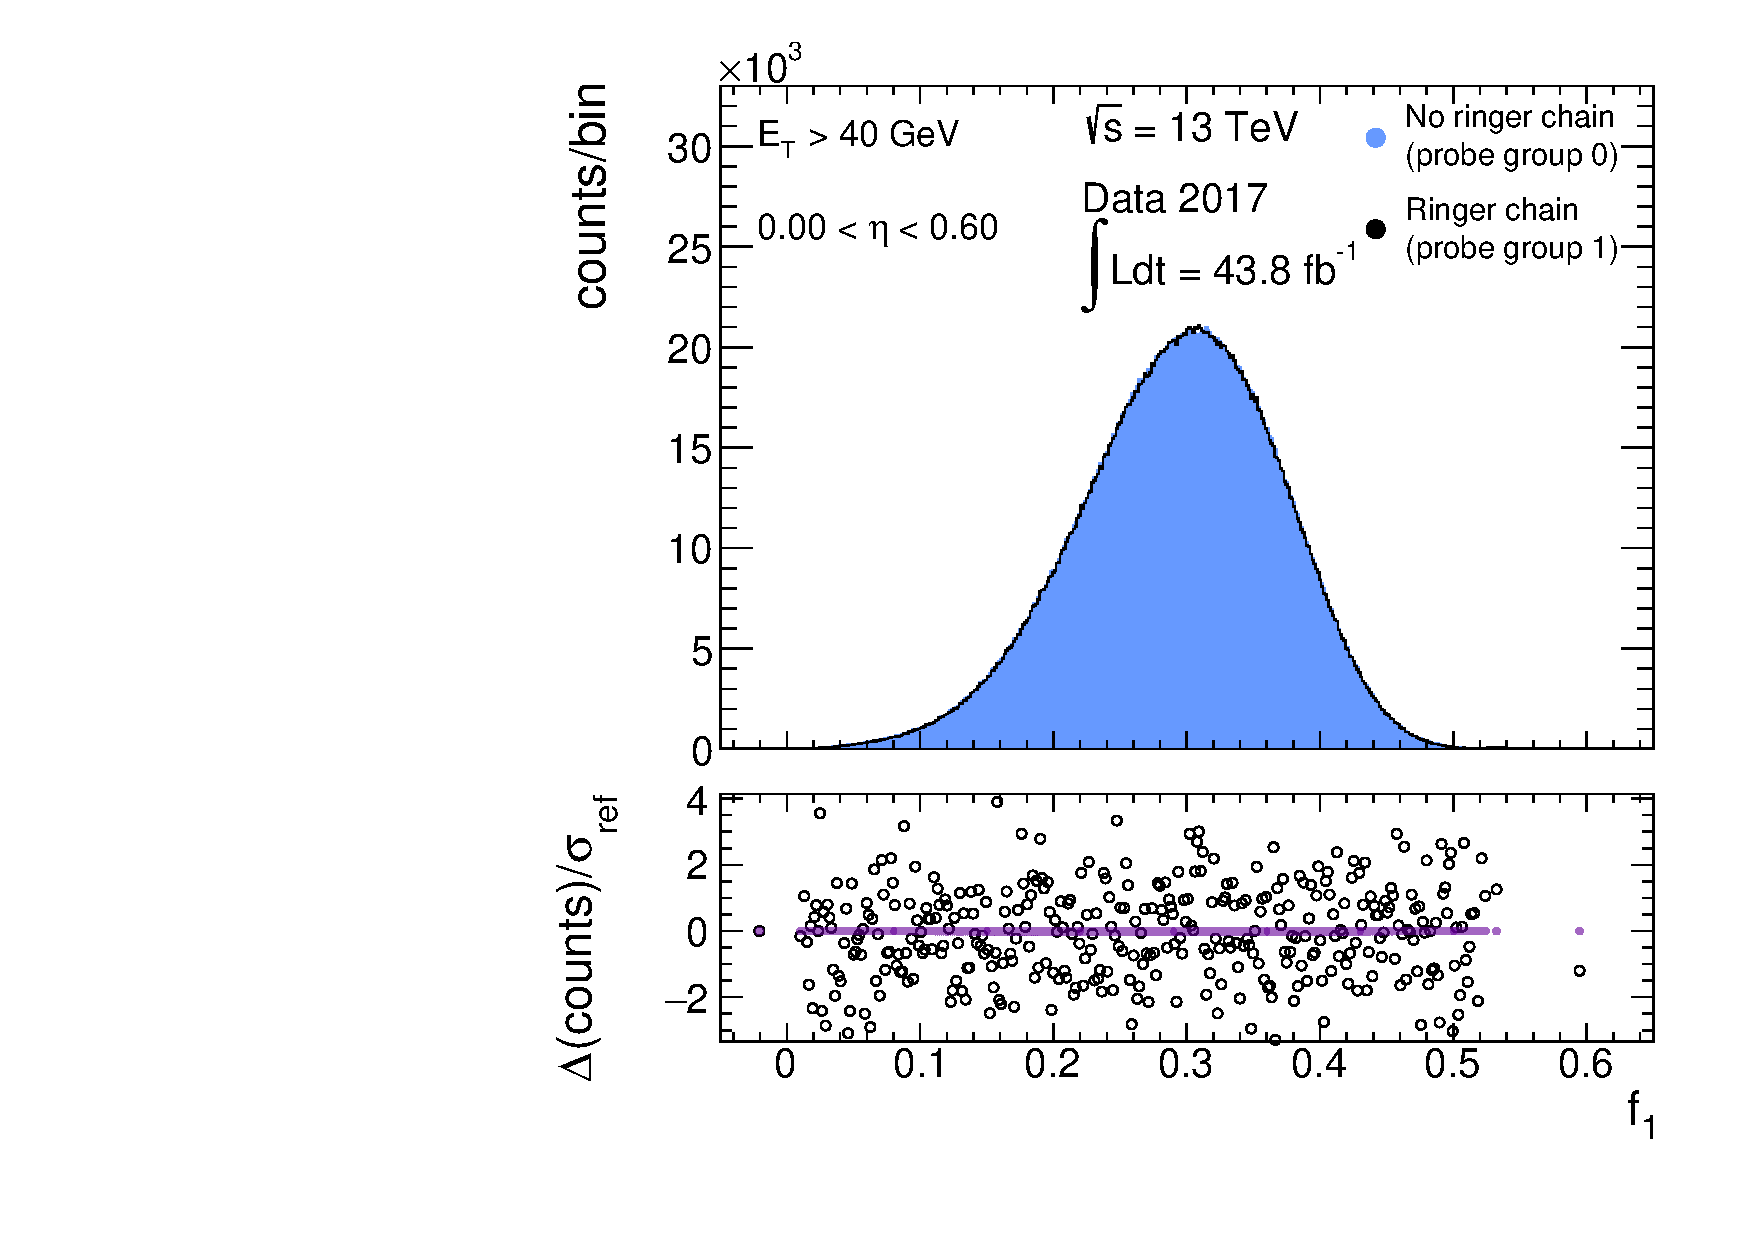
\includegraphics[width=\textwidth]{appendices/figures/noAdjustment/marginal_nosplit/e28_MergedRuns/base_new/el_f1_et40eta0_00_sigma_base_new.pdf}
\caption{}%
\label{fig:gof_f1}
\end{subfigure}
\hfill
\begin{subfigure}[c]{.48\textwidth}
\centering
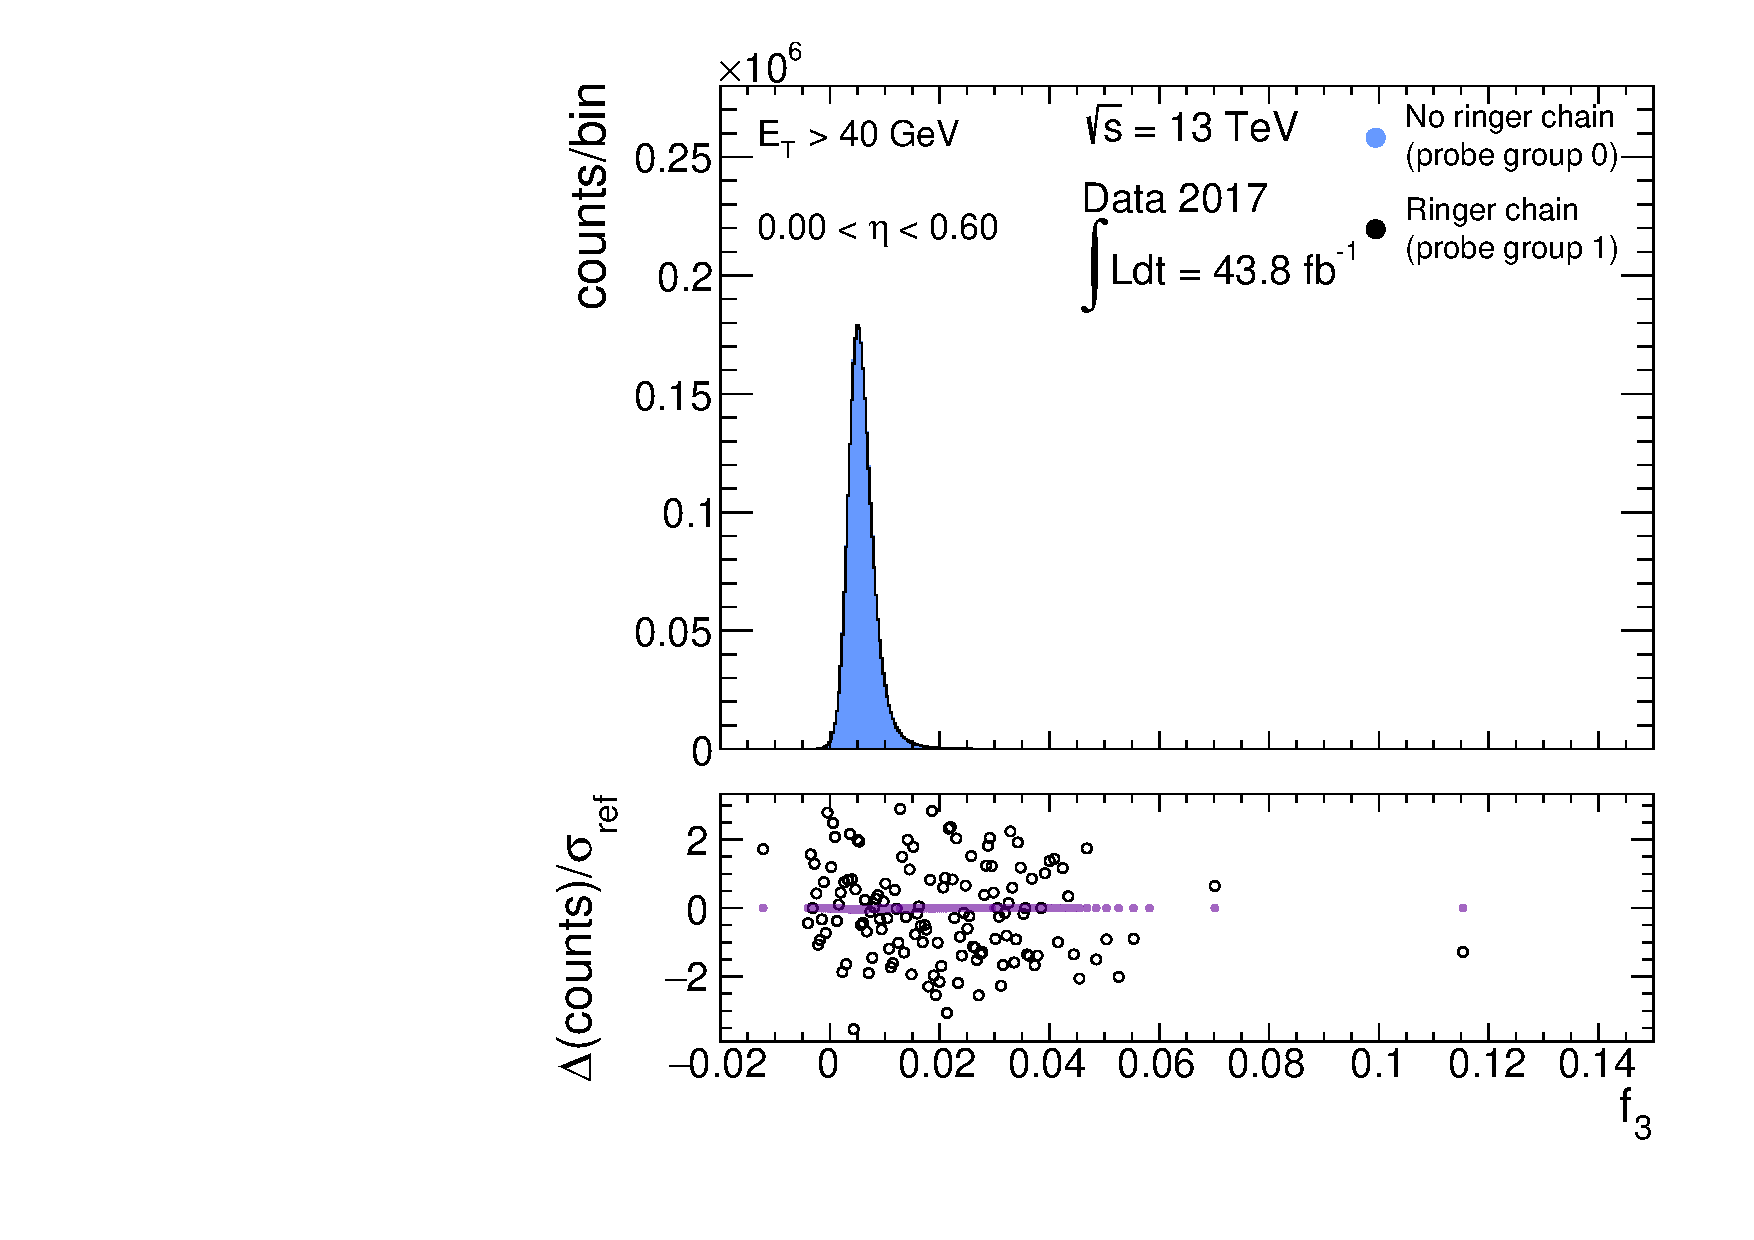
\includegraphics[width=\textwidth]{appendices/figures/noAdjustment/marginal_nosplit/e28_MergedRuns/base_new/el_f3_et40eta0_00_sigma_base_new.pdf}
\caption{}%
\label{fig:gof_f3}
\end{subfigure} \\
\caption{%
Top: Histogram profiles for the calorimetry variables employed in the offline
likelihood in the $\et>\SI{40}{\GeV}$ and $0.00<\abseta{}<0.80$ regions using
the trigger without \rnn{} (blue area) and the trigger with \rnn{} (black line).
Bottom: residual contributions using as statistics $\chi^s$
(equation~\ref{eq:signed_chi}, in black) and the expected model for no
distortion (equation~\ref{eq:expected_residual}) w.r.t.\@ the reference.
}%
\label{fig:gof_calo}
\end{center}
\end{figure}

\FloatBarrier
\subsubsection{Pseudo-Experiment Results}\label{top:agreement_pseudo_results}

Both homogeneity and goodness-of-fit tests showed that any alteration in the
profiles due to systematic effects coming from trigger configuration are
negligible with respect to the magnitude of statistical fluctuations. In this
section, we dedicate to studying the cases where the triggers \emph{disagree} in
order to get more insight on their systematic impact in the derivation of the
likelihood pdfs regardless of its relevance.

Despite the usage of full 2017 data and the disagreement between the two
triggers, the homogeneity hypothesis for most variables (\rphi{} \fI{},
\eratio{} and \weta{}) is not rejected at a 0.05 confidence level. It shows that
the overall alteration in the profiles due to the trigger configuration is not
statistically strong for these variables even when considering only the
disagreement samples. Particularly, that is not the case for the \reta{} and
\rhad{} variables where the homogeneity hypothesis is discarded. For \reta{}, it
is possible to observe that the trigger with \rnn{} is likely to collect
more \tnp{} pairs with probe samples whose \reta{} values are greater than 0.959
and less otherwise with respect to triggering without it. Similarly, the trigger
with \rnn{} seems to be biased to collect less samples with \rhad{} above
values around \SI{1.75}{\textperthousand} and more otherwise with respect to its
duplicated counterpart. Although not being statistically significant, a similar
behavior may be present in \eratio{} and \rphi{}, where \rnn{} trigger displays
a slight shift toward unitary values.

Interestingly, these results are similar to those found in the quadrant analysis
(Section~\ref{top:quadrant_results}).  However, the reason for the single
electron trigger selection configuration applied on the tag to affect the probe
profiles is unclear. One possible explanation would be some correlation level
between the ID variables of the two Z electrons.

\begin{figure}[hbt]
\begin{center}
\begin{subfigure}[c]{.48\textwidth}
\centering
\includegraphics[width=\textwidth]{appendices/figures/noAdjustment/marginal_mutually_exclusive/e28_MergedRuns_mutuallyExclusive/bonly_nonly/el_reta_et40eta0_00_kldivergence_bonly_nonly.pdf}
\caption{}%
\label{fig:pseudo_reta}
\end{subfigure}
\hfill
\begin{subfigure}[c]{.48\textwidth}
\centering
\includegraphics[width=\textwidth]{appendices/figures/noAdjustment/marginal_mutually_exclusive/e28_MergedRuns_mutuallyExclusive/bonly_nonly/el_rphi_et40eta0_00_kldivergence_bonly_nonly.pdf}
\caption{}%
\label{fig:pseudo_rphi}
\end{subfigure} \\
\begin{subfigure}[c]{.48\textwidth}
\centering
\includegraphics[width=\textwidth]{appendices/figures/noAdjustment/marginal_mutually_exclusive/e28_MergedRuns_mutuallyExclusive/bonly_nonly/el_eratio_et40eta0_00_kldivergence_bonly_nonly.pdf}
\caption{}%
\label{fig:pseudo_eratio}
\end{subfigure}
\hfill
\begin{subfigure}[c]{.48\textwidth}
\centering
\includegraphics[width=\textwidth]{appendices/figures/noAdjustment/marginal_mutually_exclusive/e28_MergedRuns_mutuallyExclusive/bonly_nonly/el_rhad_et40eta0_00_kldivergence_bonly_nonly.pdf}
\caption{}%
\label{fig:pseudo_rhad}
\end{subfigure} \\
\end{center}
\end{figure}%
\begin{figure}[t]\ContinuedFloat
\begin{center}
\hspace*{\fill}
\begin{subfigure}[c]{.48\textwidth}
\centering
\includegraphics[width=\textwidth]{appendices/figures/noAdjustment/marginal_mutually_exclusive/e28_MergedRuns_mutuallyExclusive/bonly_nonly/el_weta2_et40eta0_00_kldivergence_bonly_nonly.pdf}
\caption{}%
\label{fig:pseudo_weta}
\end{subfigure}
\hspace*{\fill} 
\begin{subfigure}[c]{.48\textwidth}
\centering
\includegraphics[width=\textwidth]{appendices/figures/noAdjustment/marginal_mutually_exclusive/e28_MergedRuns_mutuallyExclusive/bonly_nonly/el_f1_et40eta0_00_kldivergence_bonly_nonly.pdf}
\caption{}%
\label{fig:pseudo_f1}
\end{subfigure}
\hfill
%\begin{subfigure}[c]{.48\textwidth}
%\centering
%\includegraphics[width=\textwidth]{noAdjustment/marginal_mutually_exclusive/e28_MergedRuns_mutuallyExclusive/bonly_nonly/el_f3_et40eta0_00_kldivergence_bonly_nonly.pdf}
%\caption{}%
%\label{fig:pseudo_f3}
%\end{subfigure} \\
\caption{The top pad shows the histogram profiles for the disagreements between
  triggering with and without \rnn{} for each calorimetry
  variable\footnotemark{} employed in the offline likelihood in the
  $\et>\SI{40}{\GeV}$ and $0.00<\abseta{}<0.80$ regions. Abscissa is weighed
  through the histogram bin size according to the bin-to-bin observed
  ($\dkl{}(b_{obs}||r_{obs})$) divergence contributions, shown in orange in the
  bottom pad. They are computed for each bin by the divergence between triggers
  with \rnn{} (square in the top pad) and without (circle). The triangles show
  the observations of the trigger with \rnn{} reweighed to have the same mass of
  the other trigger.  On the top left, the observed \dkl{} between the two
  profiles is shown in the red line.  The mean and standard deviation of the
  pseudo-experiment \dkl{} distribution followed by the corresponding p-value is
  in the next line. The unidimensional distribution of the pseudo-experiments
  are in blue and red for each bin. The distribution for the bin-to-bin \dkl{}
  contributions is in grey in the bottom pad. Dashed lines indicate the bin
  boundaries and the values on top are the corresponding bin centers.}%
\label{fig:pseudo_calo}
\end{center}
\end{figure}

\footnotetext{\fIII{} is not included due to technical issues.}

\FloatBarrier
